\documentclass{article}
\usepackage{graphicx}

\usepackage[english]{babel}

\begin{document}

cloud data
 \begin{table}
 \small
 \begin{tabular}{|c|c|c|c|c|c|c|} 
 \hline 
 Case&Read File&Threads  & \# of & Total & \# of  &  $T_C$  \\ 
     & Size (MB) & per Task & Tasks & Cores &  VM's & seconds \\ 
\hline
c1 & 800  &8 & 1 &  8 & 1 &2001  \\\hline
c2 & 400 &4 & 2 &  8 & 1 &921 \\\hline
c3 & 200 &2 & 4 &  8 & 1 &569 \\\hline
c4 & 100 &1 & 8 &  8 & 1 &366 \\\hline

\hline

 \end{tabular}

 \caption{ The number of index files used for this measurement is 10(1.7 GB).
   In all cases the input and output data resides on VM itself.  VM in
   case c1 c2, c3, c4 are of type c1.xlarge }
  \label{table:cloud-VM} 
\end{table}






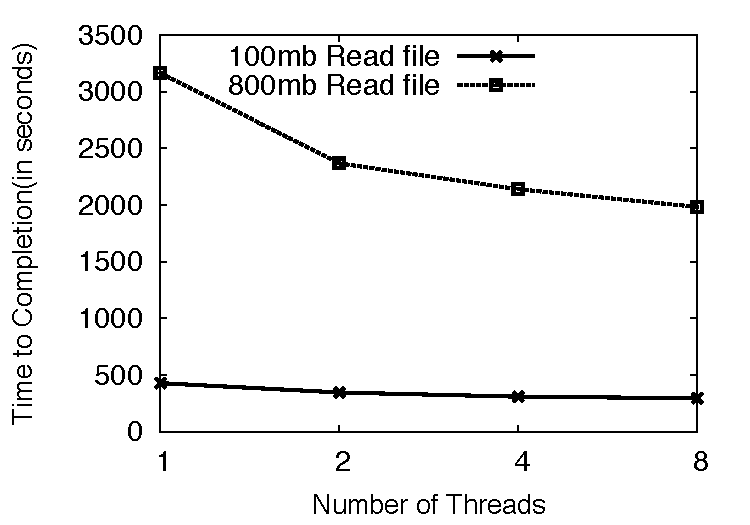
\includegraphics[scale=0.66]{../figures/cloud_threadsvstime.pdf} 



\end{document}

